\section{双平方根方程的意义}
\label{sec:3.4}

双平方根方程具有石油勘探地震数据处理中大多数非统计方法方面的特点.这种在前一
节中导出的方程颇不易于理解,因为它是一种在四维空间$(z,s,g,t)$中的算子。我们将
通过各种具体应用来对它进行探讨,在各该应用中它均是一种较低维空间中的问题。在本节
中,速度横向变化将忽略不计(因为事情本来就够复杂的了,要考虑它就更棘手了)。讨论
就从下列二式开始:

\begin{subequations}
\begin{equation}
\frac{dU}{dz}=-\frac{i\omega}{v}[\sqrt{1-G^2}+\sqrt{1-S^2}]U
\label{eq:ex3.4.1a}
\end{equation}
\begin{equation}
\frac{dU}{dz}=-\frac{i\omega}{v}[\sqrt{1-(Y+H)^2}+\sqrt{1-(Y-H)^2}]U
\label{eq:ex3.4.1b}
\end{equation}
\label{eq:ex3.4.1}
\end{subequations}

\subsection{零炮检距偏移$(H=0)$}
\label{sec:3.4.1}

降低\ref{eq:ex3.4.1b}之维数的一种办法就是直接令$H=0$,于是两个平方根变得相同,从而
可将它们合并,得出熟悉的旁轴方程

\begin{equation}
\frac{dU}{dz}=i\omega\frac{2}{v}\sqrt{1-\frac{v^2k_y^2}{4\omega^2}}
\label{eq:ex3.4.2}
\end{equation}

在式\ref{eq:ex3.4.2}中出现岩石速度的两个地方,该岩石速度均应除以2,这是由于为使野外资料
与爆炸反射面模型相应,就需要使岩石速度减半。所以不论我们作过了什么,只要是令$H=0$,
我们就得到在第一章中使用过的方程了。令$H=0$就使观测排列延拓概念在作用上有等价于
爆炸反射面概念的效果了。

\subsection{零倾角叠加$(Y=0)$}
\label{sec:3.4.2}

处理炮检距$h$的时候,通常假设地层是水平成层的,从而观测结果将与中心点$y$无关。除
了或换句话说,除以外,采用这样一种地层模型时,所有遍及$y$之数据资料的
Fourier变换均将为零。当$Y=0$时,式\ref{eq:ex3.4.1}中的两个平方根又变得相等,因而所得方
程再一次成为旁轴方程

\begin{equation}
\frac{dU}{dz}=i\omega\frac{2}{v}\sqrt{1-\frac{v^2k_h^2}{4\omega^2}}
\label{eq:ex3.4.3}
\end{equation}

利用这个方程将双曲面从地表向下延拓时,可发现双曲面随着深度之增大而蜷缩,直至达到
出现最佳聚焦的正确深度,这种情形如图\ref{fig:ofs/dc2}所示。

各波均在零炮检距时出现最佳聚焦。出现聚焦代表向下延拓达到目的,这时,向下延拓
正好到达一个反射面。对于正位于反射面之上的自激自收点的情形,是在零值旅行时间上的
反射最强。采集$t=0$时在零炮检距上的值并放弃其余炮检距上的值,是消除干扰的一种途径
(实际上,这就是一种限制干扰影响的方法)。粗略地说,这同沿着原始资料上的双曲线轨
跡进行求和的常规处理过程就是一回事。很自然,向下延拓处理时采用的波速最接近于地层
速度时,求和可望达到最隹状态。以后就将利用炮检距空间来测定速度。


\subsection{常规处理---近似分离法}
\label{sec:3.4.3}

将式\ref{eq:ex3.4.1b}括号中的算子在形式上定义为双平方根算子(DSR算子)
\begin{equation}
\text{DSR}(Y,H)=\sqrt{1-(Y+H)^2}+\sqrt{1-(Y-H)^2}
\label{eq:ex3.4.4}
\end{equation}

\begin{figure}[H]
\centering
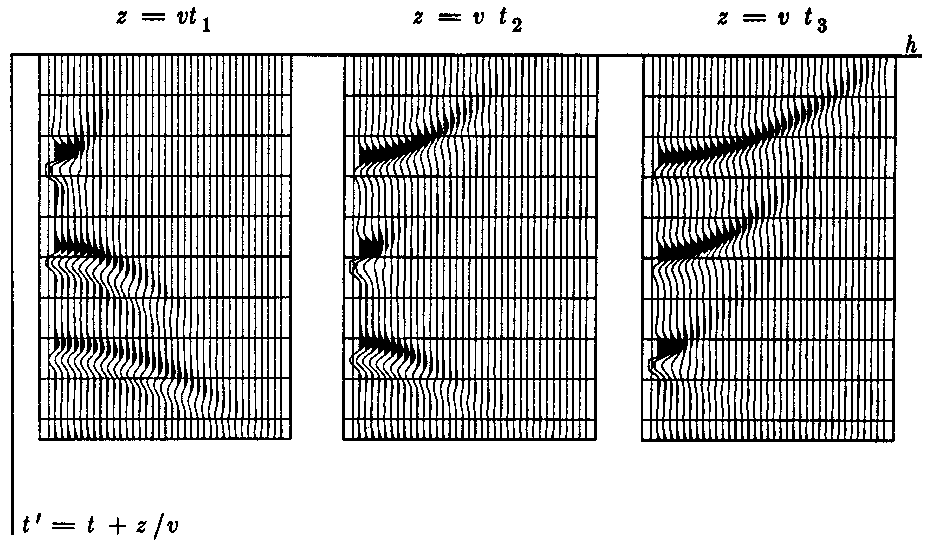
\includegraphics[width=0.65\textwidth]{ofs/dc2}
\caption[chervon]{采用三层的地层模型时,共中心点道集为三个双曲面。连续图形表示
向下延拓相继达到出现最佳聚焦时的深度}
\label{fig:ofs/dc2}
\end{figure}

在Fourie空间内,向下延拓是用相移因子$exp(i\omega \text{DSR}\frac{z}{v})$完成的。

采用这种算子有一个严重问题,无法将它分离成为一个炮检距算子与一个中心点算子之
和。不可分离的意思是,式\ref{eq:ex3.4.4}的Taylor级数展开中包含有像$Y^2H^2$这样的项,不能
把这样一些项表示成$Y$的一个函数加上$H$的一个函数,不可分离性是数据处理工作中的灾
难,它暗示着偏移与叠加必须同时完成而不能前后相继完成。要恢复纯粹的可分离性,其唯
一的途径就是回到$S$与$G$的空间中去(那可是远离常规处理的变化剧烈的抉择,我们将在以
后再转而讨论它)。

让我们回顾一下有关可分离性的一般性问题。为使算子$\sqrt{1-X^2-Y^2}$能近似分离,显
而易见的途径就是进行Taylor级数展开,然后略去所有交叉项,更精确的近似是
$\sqrt{1-X^2}+\sqrt{1-Y^2}-1$,它在$X=0$时准确地拟合于所有的$Y$,而在$Y=0$时则准确地拟合于所有的
$X$;把这个思想应用于双平方根算子,得

\begin{subequations}
\begin{equation}
\text{SEP}(Y,H)=2+[\text{DSR}(Y,0)-2]+[\text{DSR}(0,H)-2]
\label{eq:ex3.4.5a}
\end{equation}
\begin{equation}
\text{SEP}(Y,H)=2[1+(\sqrt{1-Y^2}-1)+(\sqrt{1-H^2}-1)]
\label{eq:ex3.4.5b}
\end{equation}


注意,在时,式\ref{eq:ex3.4.5}就等于双平方根算子;在$Y=0$时,该式也是等于双平方根
算子,仅当$H$与$Y$二者均非零时,SEP才不同于DSR。

式\ref{eq:ex3.4.5}分解成三个算子之和,能提供一种类似二维Fourier积分核$exp(ik_yy+ik_hh)$
所能提供的好处,该积分核具有的相位是由两部分之和所组成,这意味着Fouriei积分能够
对$y$或$h$按内嵌套循环进行处理。所以利用SEP进行向下延拓时,可以如式\ref{eq:ex3.4.1b}
所暗示的那样在$(k_h,k_y)$空间内完成,或者我们可以选定Fouriei变换,以适当的嵌套循环运算方
法变换至$(h,k_y)$、$(k_h,y)$或者$(y,h)$。

对式\ref{eq:ex3.4.5b}中的三项各取一个熟悉的名字是可带来方便的。第一项与时间深度转换
有关,第二项与偏移有关,第三项与正常时差有关;
\begin{equation}
\text{SEP}(Y,H)=\text{TD}+\text{MIG}(Y)+\text{NMO}(H)
\label{eq:ex3.4.5c}
\end{equation}
\label{eq:ex3.4.5}
\end{subequations}

可以把式\ref{eq:ex3.4.5}形式的近似解释为“标准处理”,标准处理中的第一步即是正常时
差校正。在式\ref{eq:ex3.4.5}中,NMO算子是将地表上的所有炮检距向下延拓为一定深度上的所
有炮检距。选择零炮检距只不过就是放弃所有其他炮检距;就同按炮检距进行叠加一样,选
择零炮检距可以减少所需考虑的数据量。

通常,被放弃的炮检距均不作偏移。相反,凡偏移之后改变叠加速度的精细处理都涉及
要对零炮检距附近的一些炮检距进行偏移。

既然SEP算子内的所有项均可相互交换,要是将它用于在叠加之前对所有炮检距迸行偏
移,那计算工作量似乎就太浪费了。梦样作所得结果将与叠后偏移完全一样。

\subsection{$H=0$的各种意义}
\label{sec:3.4.4}

时差算子$2H/v$有各种不同的形式:
\begin{equation*}
\frac{dt}{dh} ----- \text{射线轨迹情形下}
\end{equation*}
\begin{equation*}
\frac{k_h}{\omega} ----- \text{Fouder变换情形下}
\end{equation*}
\begin{equation*}
\partial_h^t=\int_{-\inf}^t dt\frac{\partial}{\partial h}-----\text{偏微分方程情形下}
\end{equation*}

互易性暗示着旅行时间〖为炮检距A的一个对称函数,从面在$h=0$时,$dt/dh$为零。在那
种意义下,把式\ref{eq:ex3.4.2}应用于零炮检距剖面看来是适宜的。更准确地说,射线轨迹表达
式严格说来只能在有一个平面波的时候才可应用。球形波阵面是由许多平面波之叠加
所形成。这时,关于$H$的Fouder变换解释要有稍许差别,而且更恰如其分。要挑选零频率
分量、即挑选地震记录道的平均值时,就令$\omega=0$;要挑选零空间频率分量,就是说,要挑选遍及
炮检距的求和,就令$k_h$=0。常规叠加可定义为沿某个双曲线轨迹遍及炮检距的积分或者求
和,直接令$k_h=0$就是挑选某个拉伸展平的双曲线轨迹,亦即速度为无限大时的双曲线。这
么一种积分或求和会接收到来自数据双曲面之顶部的主要影响,在该顶部,同相轴开始与进
行积分或求和所沿的水平直线相切。(由于若干历史原因,这样一种数据求和往往称为垂直
叠加)。在时差还没达到等于半波长之前,对积分的主要影响大多数是来自双曲线顶部邻近
的区域,称作Fresnel带的这种区域之宽度是影响该积分的主要因素。Fresnel带的概念已
在\ref{sec:1.2}节内介绍过了。图\ref{fig:ofs/denmark}所示是从一张野外剖面提取出的Fresnel带。

\begin{figure}[H]
\centering
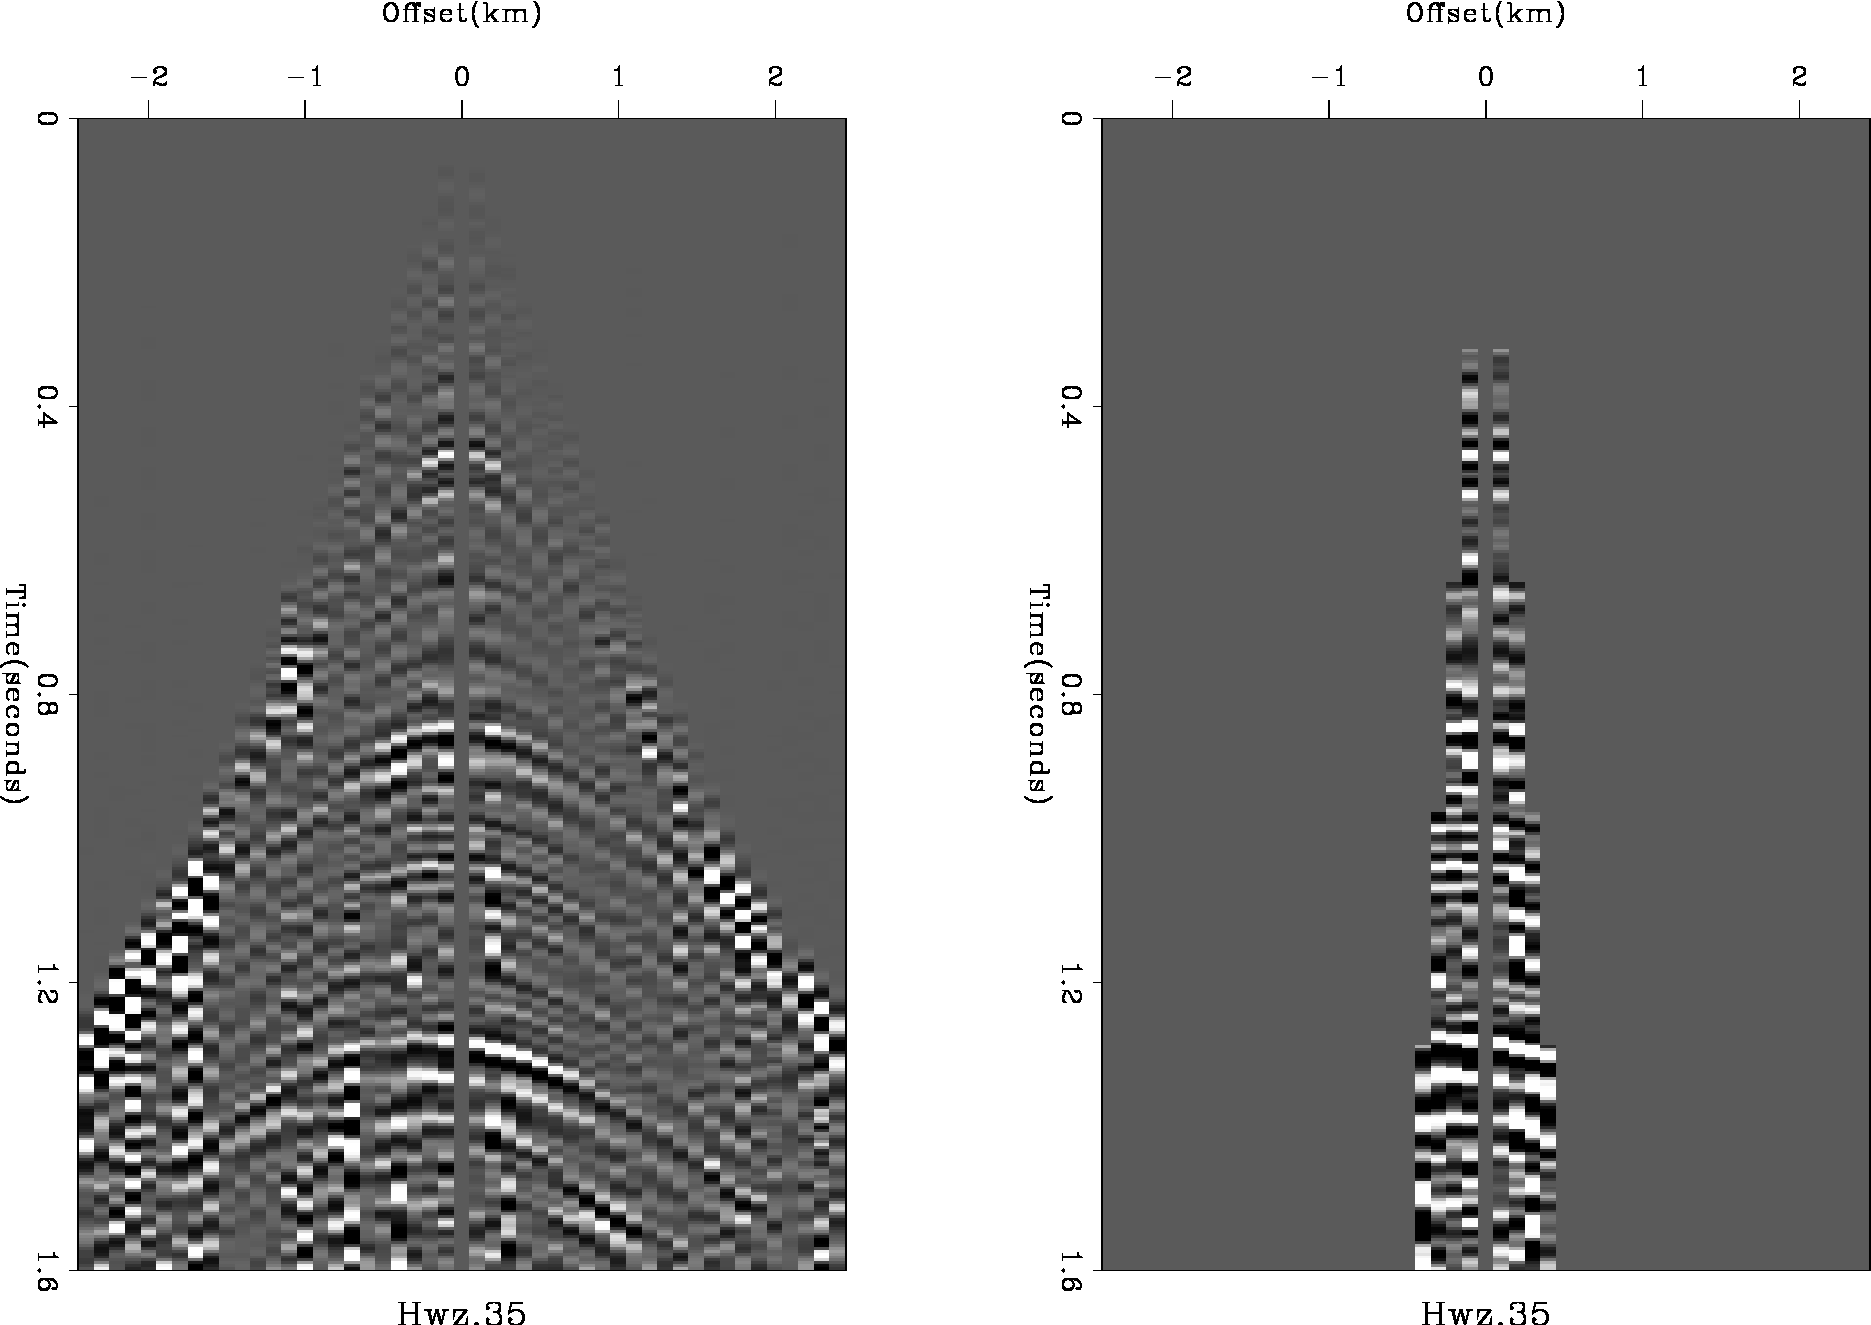
\includegraphics[width=0.65\textwidth]{ofs/denmark}
\caption[denmark]{丹麦某地区的陆地剖面(左图),由左图提取出并加以重新显示的
Fresnel带(右图)}
\label{fig:ofs/denmark}
\end{figure}
